\documentclass[conference]{IEEEtran}
\IEEEoverridecommandlockouts
\usepackage{cite}
\usepackage{amsmath,amssymb,amsfonts}
\usepackage{algorithmic}
\usepackage{graphicx}
% Ensure LaTeX can find images whether this file is compiled standalone or included from project root.
% Prefer project-level `images/` folder first (Overleaf compiles from project root).
\graphicspath{{images/}{./images/}{./}{../images/}}
% Recognize common image extensions (helps pdfLaTeX/Overleaf find images)
\DeclareGraphicsExtensions{.pdf,.png,.jpg,.jpeg}
\usepackage{textcomp}
\usepackage{xcolor}
\usepackage{url}
% fontspec requires XeLaTeX/LuaLaTeX. Use it only when available; otherwise fall back to a
% Times-like package compatible with pdfLaTeX to avoid Overleaf compile errors.
\usepackage{iftex}
\ifXeTeX
    \usepackage{fontspec}
    \setmainfont{Times New Roman}
\else
    % pdfLaTeX fallback: use mathptmx (Times-like text and math)
    \usepackage{mathptmx}
\fi
\usepackage{tikz}
\usepackage{pgfplots}
\usepackage{float}
\usepackage{stfloats}
\usepackage{placeins}
\raggedbottom
\usetikzlibrary{positioning,calc,backgrounds}
\usepackage{enumitem}
\pgfplotsset{compat=1.18}
\usetikzlibrary{arrows.meta,positioning,shapes.geometric,calc,shapes}
% Chuẩn hoá float placement cho IEEEtran
\makeatletter
\setcounter{topnumber}{3}
\setcounter{bottomnumber}{1}
\setcounter{totalnumber}{4}
\renewcommand{\topfraction}{0.85}
\renewcommand{\bottomfraction}{0.15}
\renewcommand{\textfraction}{0.1}
\makeatother
\def\BibTeX{{\rm B\kern-.05em{\sc i\kern-.025em b}\kern-.08emem
    T\kern-.1667em\lower.7ex\hbox{E}\kern-.125emX}}
\begin{document}
\title{\textbf{Hệ Thống AI-Agent Cho Nền Tảng Đồ Cũ:\\MVP FastAPI + BERT4Rec Cho Gợi Ý Tuần Tự}}
\author{\IEEEauthorblockN{\textbf{Nguyễn Phương Nam}}
\textit{DaiNam University} \\
\textit{Hanoi, Vietnam} \\
\textit{Email: namnamnamaa8@gmail.com} \\
}
\maketitle
\begin{abstract}
Bài viết này trình bày phiên bản \textit{minimum viable product} (MVP) của AI-Agent cho nền tảng thương mai điện tử Second-hand Web VietNam. Trọng tâm hiện tại là dịch vụ \textbf{FastAPI} gắn với mô hình tuần tự \textbf{BERT4Rec} để trả gợi ý Top-K theo lịch sử người dùng; khi thiếu dữ liệu, chatbot trả lời mẫu và hướng dẫn đăng nhập. Pipeline sử dụng bộ dữ liệu gồm \textbf{95 sản phẩm}, \textbf{2\,608 người dùng} và \textbf{18\,301 tương tác} phân bố theo sự kiện (view 32.7\%, click 22.9\%, purchase 16.3\%, add-to-cart 15.9\%, reject 6.4\%, out 5.8\%), được chuẩn hoá bằng RecBole. Hệ thống hỗ trợ nạp checkpoint động, giám sát qua \texttt{/health} và inference trên CPU \textasciitilde0.5~s mỗi yêu cầu (4~vCPU). Lần huấn luyện thực tế trên 11/11/2025 cho thấy mô hình đạt \textbf{Recall@10 = 0.9843}, \textbf{NDCG@10 = 0.968} và \textbf{MRR@10 = 0.8637}, chứng tỏ thuật toán sẵn sàng triển khai thực tế. Chúng tôi mô tả kiến trúc, luồng dữ liệu, bài học vận hành, kết quả hiệu năng và nêu rõ các hạng mục đang nằm trong lộ trình (\textit{Tool Router}, \textit{RAG}, \textit{LLM}).
\end{abstract}
\begin{IEEEkeywords}
AI-Agent, FastAPI, BERT4Rec, sequential recommendation, second-hand marketplace
\end{IEEEkeywords}
\section{Giới Thiệu}

Thị trường thương mại điện tử tại Việt Nam tăng trưởng mạnh nhờ mô hình kinh tế tuần hoàn và sự phổ biến của các nền tảng mạng xã hội. Tuy nhiên, trải nghiệm người dùng vẫn chịu ảnh hưởng bởi ba yếu tố: \textit{(i)} dữ liệu hành vi rời rạc giữa nhiều dịch vụ, \textit{(ii)} thiếu công cụ tư vấn tự động đáng tin cậy, và \textit{(iii)} hạ tầng AI nội bộ còn hạn chế khiến việc triển khai các mô hình lớn gặp khó khăn. Hầu hết hệ thống hiện tại dựa trên tìm kiếm từ khóa hoặc bộ lọc đơn giản, khiến người dùng mất thời gian và nhân viên hỗ trợ phải xử lý lặp lại.
Để giải quyết, chúng tôi phát triển \textbf{AI-Agent} như mô-đun trung tâm trong hệ sinh thái Second-hand Web VietNam. Phiên bản MVP tập trung vào gateway \textbf{FastAPI} và mô hình tuần tự \textbf{BERT4Rec}: gateway nhận yêu cầu, nhận diện ý định dựa trên từ khóa, gọi recommender để trả gợi ý hoặc trả lời mẫu khi chưa đủ dữ liệu. Các thành phần nâng cao như Tool Router, RAG tra cứu tri thức và chatbot LLM hiện nằm trong lộ trình mở rộng. Hệ thống hướng đến:
\begin{itemize}
    \item \textbf{Chuẩn hoá dữ liệu}: chuyển log hành vi rời rạc thành chuỗi tương tác ngắn hạn phù hợp với RecBole.
    \item \textbf{Vận hành ổn định}: duy trì dịch vụ gợi ý với cơ chế reload checkpoint và fallback khi mô hình chưa sẵn sàng.
    \item \textbf{Khả năng mở rộng}: mở đường cho các mô-đun điều phối nâng cao (Tool Router/RAG) mà không phải thay đổi giao diện API.
\end{itemize}
Những đóng góp chính của bài viết này:
\begin{enumerate}
    \item \textbf{Kiến trúc mở}: mô tả cách triển khai phiên bản đầu tiên chỉ với FastAPI + BERT4Rec nhưng vẫn duy trì giao diện mở để gắn thêm Tool Router/RAG sau này.
    \item \textbf{Pipeline dữ liệu}: trình bày chi tiết bộ dữ liệu thực tế (95 sản phẩm, 2\,608 người dùng, 18\,301 tương tác với phân bố sự kiện: view 32.7\%, click 22.9\%, purchase 16.3\%, add-to-cart 15.9\%, reject 6.4\%, out 5.8\%) cùng quy trình huấn luyện, nạp checkpoint và vận hành inference CPU. Lần huấn luyện thực tế trên 11/11/2025 lưu lại các log chi tiết và checkpoint đã được kiểm chứng.
    \item \textbf{Lộ trình phát triển}: phân tích những hạn chế hiện tại (thiếu dữ liệu thật, chưa đo lường người dùng, chưa có RAG/LLM) và kế hoạch mở rộng trong các quý tới.
\end{enumerate}

\noindent \textbf{Tổ chức bài viết}: Phần còn lại được cấu trúc theo luồng logic của hệ thống: (1) Phần \textit{Dữ Liệu \& Tập Dữ Liệu} giới thiệu bộ dữ liệu thực tế gồm 95 sản phẩm, 2\,608 người dùng, 18\,301 tương tác; (2) Phần \textit{Kiến Trúc Hệ Thống} mô tả ba lớp: Frontend, Service/Backend, Data \& Intelligence; (3) Phần \textit{Phương Pháp} chi tiết quá trình tiền xử lý, huấn luyện BERT4Rec, và quy trình hội thoại FastAPI; (4) Phần \textit{Đánh Giá Thực Nghiệm} trình bày kết quả huấn luyện (Recall@10=0.9843, NDCG@10=0.968), phân tích hiệu năng inference, và tóm tắt trạng thái triển khai; (5) Cuối cùng, phần \textit{Thảo Luận} và \textit{Kết Luận} đánh giá ưu điểm, hạn chế và hướng phát triển tiếp theo.
\section{{Công Trình Liên Quan}}
Các hệ gợi ý TMĐT phổ biến dựa trên collaborative filtering hoặc deep neural recommender \cite{b3}, trong khi chatbot thương mại thường dựa trên rule-based. Nghiên cứu gần đây cho thấy LLM kết hợp vector embeddings giúp hiểu ngữ nghĩa tốt hơn \cite{b2,b5}. Tuy nhiên, ít công trình tập trung vào bối cảnh đồ cũ tại Việt Nam. Hệ thống của chúng tôi kế thừa hướng kết hợp LLM + semantic search, đồng thời tận dụng RecBole/BERT4Rec để xử lý chuỗi hành vi ngắn hạn.
\section{{Dữ Liệu \& Tập Dữ Liệu}}
\subsection{{Mô Tả Bộ Dữ Liệu}}
Để phát triển và kiểm chứng hệ thống AI-Agent, nhóm xây dựng bộ dữ liệu từ dữ liệu thực tế của nền tảng Second-hand Web VietNam, gồm:

\begin{itemize}
    \item \textbf{Catalog sản phẩm}: 95 sản phẩm thực tế từ thư mục hiện có, mỗi sản phẩm có thông tin: ID, tên, danh mục, giá, mô tả.
    \item \textbf{Người dùng}: 2\,608 người dùng độc lập có lịch sử tương tác.
    \item \textbf{Tương tác (Interactions)}: 18\,301 sự kiện hành vi được ghi lại, bao gồm 6 loại sự kiện chính:
    \begin{itemize}
        \item \textbf{view} (xem): 5\,978 sự kiện (32.7\%) — người dùng xem chi tiết sản phẩm.
        \item \textbf{click} (nhấp): 4\,197 sự kiện (22.9\%) — tương tác gián tiếp (click button, filter).
        \item \textbf{purchase} (mua): 2\,981 sự kiện (16.3\%) — giao dịch hoàn tất.
        \item \textbf{add-to-cart} (thêm giỏ): 2\,915 sự kiện (15.9\%) — sản phẩm được đưa vào giỏ hàng.
        \item \textbf{reject} (từ chối): 1\,168 sự kiện (6.4\%) — người dùng bỏ qua/xóa khỏi giỏ.
        \item \textbf{out} (ra khỏi): 1\,062 sự kiện (5.8\%) — kết thúc phiên mà không mua.
    \end{itemize}
\end{itemize}

Hình~\ref{fig:dataset-dist} dưới đây thể hiện phân bố sự kiện, cho thấy tính cân bằng hợp lý giữa các loại hành vi trong e-commerce điển hình.

\begin{figure}[H]
    \centering
    \begin{tikzpicture}
        \begin{axis}[
            ybar,
            bar width=10pt,
            width=0.9\linewidth,
            height=4.2cm,
            ylabel={Số lượng sự kiện},
            symbolic x coords={view,click,purchase,add-to-cart,reject,out},
            xtick=data,
            x tick label style={rotate=20,anchor=east},
            ymin=0,
            ymax=7000,
            nodes near coords,
            nodes near coords align={vertical},
            every node near coord/.append style={font=\scriptsize},
            enlarge x limits=0.05
        ]
            \addplot[fill=blue!50] coordinates {
                (view,5978)
                (click,4197)
                (purchase,2981)
                (add-to-cart,2915)
                (reject,1168)
                (out,1062)
            };
        \end{axis}
    \end{tikzpicture}
    \caption{Phân bố sự kiện hành vi: 18\,301 tương tác thực tế từ 2\,608 người dùng trên 95 sản phẩm. Các sự kiện phản ánh hành vi điển hình của e-commerce: view chiếm 32.7\%, click 22.9\%, purchase 16.3\%, add-to-cart 15.9\%, reject 6.4\%, out 5.8\%.}
    \label{fig:dataset-dist}
\end{figure}

\subsection{{Xử Lý và Chuẩn Bị}}
Bộ dữ liệu được chuẩn bị qua 3 bước chính:
\begin{enumerate}
    \item \textbf{Chuẩn hoá Catalog}: Script \texttt{normalize\_catalog\_data.py} làm sạch và chuẩn hoá trường dữ liệu sản phẩm.
    \item \textbf{Sinh Hành Vi}: Script \texttt{user\_behavior\_advanced.py} tạo chuỗi tương tác (sequences) từ log hành vi thô, bao gồm dấu thời gian và loại sự kiện.
    \item \textbf{Chuyển Định Dạng}: Script \texttt{prepare\_interactions\_for\_recbole.py} chuyển đổi sang định dạng \texttt{.inter} của RecBole.
\end{enumerate}

Dữ liệu cuối cùng được chia ngẫu nhiên với tỷ lệ \textbf{80\% training}, \textbf{10\% validation}, \textbf{10\% test}. Ma trận tương tác có độ thưa thớt (**sparsity**) là 92.7\%, điều này phổ biến trong các hệ e-commerce thực tế và phù hợp cho việc kiểm chứng các mô hình gợi ý tuần tự.

\section{{Kiến Trúc Hệ Thống}}
Hệ thống được tổ chức thành ba lớp chính, mỗi lớp được thiết kế để tối ưu hoá một nhóm chức năng cụ thể và đồng thời giảm sự phụ thuộc chặt giữa các thành phần nhằm tăng khả năng mở rộng, dễ bảo trì và khả năng tích hợp về sau.

\paragraph{1) Frontend Layer}
Frontend chịu trách nhiệm tương tác trực tiếp với người dùng cuối và thu thập ngữ cảnh phiên (session context). Các thành phần chính bao gồm: (i) chatbot widget nổi trên trang sản phẩm; (ii) automation triggers (ví dụ: phát hiện hành vi "bỏ giỏ", tìm kiếm nhiều lần nhưng không mua, duyệt sản phẩm nhiều lần trong một phiên); (iii) thu thập metadata như user-agent, ngôn ngữ, giờ địa phương và các sự kiện UI (click, view, add-to-cart). Frontend gửi các payload JSON chuẩn tới gateway theo contract đã định (các trường bắt buộc / tuỳ chọn rõ ràng). 

\paragraph{2) Service / Backend Layer}
Tầng này do FastAPI gateway đảm nhiệm. Gateway thực hiện các nhiệm vụ sau: xác thực và thẩm định payload, phát hiện intent bằng bộ rules/từ khoá sơ bộ, kiểm tra trạng thái model (MODEL_READY) qua healthchecks.

Về mặt thiết kế, gateway cung cấp một contract API cố định (ví dụ \texttt{/chat}, \texttt{/health}, \texttt{/internal/reload}) để Frontend và các hệ thống khác không cần biết nội bộ có bao nhiêu công cụ hoặc mô-đun; khi Tool Router được tích hợp, gateway sẽ chỉ điều hướng yêu cầu đến Router thay vì trực tiếp gọi BERT4Rec — điều này giữ nguyên backward compatibility cho các client hiện có.

\paragraph{3) Data \& Intelligence Layer}
Tầng dữ liệu và trí tuệ nhân tạo bao gồm các dịch vụ lưu trữ và mô-đun ML: hiện tại hệ thống chạy BERT4Rec (RecBole + PyTorch) dùng file CSV và checkpoint \texttt{.pth} cho inference. Các logs inference, logs training và dataset được lưu sẵn để phục vụ phân tích và tái huấn luyện định kỳ. Kiến trúc cũng dự phòng các thành phần mở rộng như RAG Search (LangChain + Qdrant) để hỗ trợ tra cứu tri thức và chatbot LLM cho các câu hỏi mở rộng; các module này được giữ ở trạng thái planned nhưng interface đã được nghĩ trước để dễ tích hợp.

\paragraph{Luồng điều phối và mở rộng}
Hiện tại gateway gọi trực tiếp BERT4Rec cho yêu cầu gợi ý. Khi cần mở rộng (phase 2), một \textit{Tool Router} sẽ được chèn giữa gateway và các backend: Router sẽ quyết định hướng luồng đến BERT4Rec, RAG, macro/FAQ hoặc kết hợp điểm (ensembling) tuỳ theo intent, độ tự tin (confidence) và trạng thái dữ liệu người dùng.
\paragraph{Vận hành, giám sát \& bảo mật}
Hệ thống tích hợp healthchecks, logging để hỗ trợ vận hành qua endpoint \texttt{/health} (trạng thái MODEL\_READY/STATUS) và inference logs (audit/retraining). Gateway áp dụng token validation, rate limiting và ghi lại mọi event. Khi người dùng tương tác (ví dụ nhấp "gợi ý"), Frontend gửi request JSON kèm session context; Gateway kiểm tra intent, xác thực user, sau đó gọi BERT4Rec để lấy Top-K hoặc trả FAQ preset khi thiếu dữ liệu. Kết quả được format Markdown/JSON; mọi event được ghi log phục vụ Behavior Analyzer và retraining pipeline.

Kiến trúc này vừa đơn giản,linh hoạt để mở rộng sang Tool Router/RAG/LLM mà không phá vỡ backward compatibility.


% ===================== FIGURE 1 — LAYOUT GỌN, THẲNG, CĂN LƯỚI (FULL-WIDTH) =====================
% Place on its own page and render full two-column width.
\FloatBarrier
\clearpage
\begin{figure*}[!t]
\centering
\begin{tikzpicture}[
    >=Stealth, thick, rounded corners, font=\small,
    x=0.75cm, y=0.75cm,
    layer/.style={draw, fill=#1, minimum width=17.5cm, inner sep=10pt, rounded corners=10pt},
    title/.style={font=\bfseries\small, align=center},
    pill/.style={draw, fill=#1, minimum width=3.2cm, minimum height=0.95cm, align=center, rounded corners=8pt},
    flow/.style={-Stealth, line width=1.0pt, shorten >=2pt, shorten <=2pt},
    dashedflow/.style={-Stealth, dashed, line width=1.0pt, shorten >=2pt, shorten <=2pt}
]

% ===== LAYERS =====
\node[layer=blue!9,  minimum height=2.6cm, label={[title,yshift=6pt]above:Frontend/User Layer}] (L1) {};
\node[layer=green!12, minimum height=4.8cm, below=1.0cm of L1, label={[title,yshift=6pt]above:AI Core (Processing)}] (L2) {};
\node[layer=purple!12,minimum height=3.0cm, below=1.0cm of L2, label={[title,yshift=6pt]above:Tool Router \& Chatbot}] (L3) {};
\node[layer=yellow!15,minimum height=3.0cm, below=1.0cm of L3, label={[title,yshift=6pt]above:Data Store}] (L4) {};

% Khóa bbox để \centering căn giữa đúng phần khối lớn
\path[use as bounding box]
  ([xshift=-0.7cm,yshift=-0.7cm]L4.south west)
  rectangle
  ([xshift= 0.7cm,yshift= 0.9cm]L1.north east);

% ==== CỘT TỌA ĐỘ (đối xứng) ====
\def\xA{-7.0}
\def\xB{-2.5}
\def\xC{ 2.5}
\def\xD{ 7.0}

% ===== L1: USER =====
\node[pill=violet!25] (w1) at ([xshift=\xA cm]L1.center) {Chatbot Widget};
\node[pill=violet!25] (w2) at ([xshift=\xB cm]L1.center) {Automation Triggers};
\node[pill=violet!25] (w3) at ([xshift=\xC cm]L1.center) {User Context};
\node[pill=violet!25] (w4) at ([xshift=\xD cm]L1.center) {Feedback Form};

% ===== L2: AI CORE =====
\node[pill=white] (m1) at ([xshift=\xA cm,yshift= 1.15cm]L2.center) {Behavior Analyzer};
\node[pill=white] (m2) at ([xshift=\xB cm,yshift= 1.15cm]L2.center) {BERT4Rec};
\node[pill=white] (m3) at ([xshift=\xC cm,yshift= 1.15cm]L2.center) {Decision Policy};
\node[pill=white, minimum width=8.8cm] (m4) at ([xshift=0cm ,yshift=-1.05cm]L2.center) {RAG Search (LangChain + VectorDB)};

% ===== L3: ROUTER & CHATBOT =====
\node[pill=white, minimum width=3.2cm] (r1) at ([xshift=\xB cm]L3.center) {Tool Router};
\node[pill=white, minimum width=3.6cm] (r2) at ([xshift=\xC cm]L3.center) {Chatbot LLM (GPT-4o / Gemini)};

% ===== L4: DATA STORE =====
\node[pill=white] (d1) at ([xshift=\xA cm]L4.center) {Logs (Redis/Postgres)};
\node[pill=white] (d2) at ([xshift=\xB cm]L4.center) {Catalog DB (Postgres)};
\node[pill=white] (d3) at ([xshift=\xC cm]L4.center) {VectorDB (Qdrant/Chroma)};
\node[pill=white] (d4) at ([xshift=\xD cm]L4.center) {Output Log};

% ===== ARROWS: USER → CORE =====
\draw[flow] (w1.south) -- (m1.north);
\draw[flow] (w2.south) -- (m2.north);
\draw[flow] (w3.south) -- (m3.north);
\draw[flow] (w4.south) -- ++(0,-0.75) |- (m4.north);

% ===== TRONG CORE =====
\draw[flow] (m1) -- node[above,yshift=1pt]{\footnotesize Auto trigger} (m2);
\draw[flow] (m2) -- node[above,yshift=1pt]{\footnotesize Điểm gợi ý} (m3);
\draw[flow] (m3.south) -- ++(0,-0.55) -- (m4.north);

% ===== CORE → ROUTER/CHATBOT =====
\draw[flow] (m4.south) -- (r1.north);
\draw[flow] (r1) -- (r2);

% ===== CHATBOT → USER (vuông góc, không đè) =====
\draw[flow] (r2.north) -- ++(0,0.85) -| (w1.north);

% ===== DATA I/O =====
\draw[flow] (m1.south) -- (d1.north);
\draw[flow] (m2.south) -- (d2.north);
\draw[flow] (m4.south) -- (d3.north);
\draw[flow] (r2.south) -- (d4.north);

% ===== FEEDBACK LOOP (gọn bên trái) =====
\draw[dashedflow] (d1.west) -- ++(-0.35,0) -- ++(0,5.4) -- ++(0.35,0)
  node[pos=0.86,left]{\footnotesize Learn again};

\end{tikzpicture}
\caption{Kiến trúc tổng thể của AI-Agent. Các khối Gateway + BERT4Rec đang vận hành; khối Tool Router, RAG và Chatbot LLM được giữ lại dưới dạng thiết kế (planned) để đảm bảo tính mở rộng trong các bản nâng cấp.}
\label{fig:architecture}
\end{figure*}
\FloatBarrier
% =================================================================

\section{{Phương Pháp}}
\subsection{{Luồng Tiền Xử Lý}}
Pipeline tại \texttt{ai-agent/data/preprocessing} gồm ba script chính được tổ chức rõ ràng như sau:
\begin{enumerate}[itemsep=0pt,topsep=0pt,parsep=0pt,partopsep=0pt]
    \item \texttt{normalize\_catalog\_data.py}: chuẩn hoá và làm sạch các trường dữ liệu trong catalog, xuất file \texttt{products.csv}.
    \item \texttt{user\_behavior\_advanced.py}: sinh chuỗi hành vi (view, click, add\_to\_cart, purchase, reject, out) kèm dấu thời gian từ các log thô.
    \item \texttt{prepare\_interactions\_for\_recbole.py}: chuyển đổi các file đã chuẩn hoá sang định dạng đầu vào của RecBole (\texttt{.inter} / cấu trúc dataset).
\end{enumerate}

Bộ dữ liệu cuối cùng chứa \textbf{95} sản phẩm, \textbf{2\,608} người dùng và \textbf{18\,301} tương tác. Dữ liệu được chia ngẫu nhiên theo tỷ lệ \textbf{80\% / 10\% / 10\%} cho train / validation / test. Phân bố các loại sự kiện là: view 32.7\% (5\,978), click 22.9\% (4\,197), purchase 16.3\% (2\,981), add-to-cart 15.9\% (2\,915), reject 6.4\% (1\,168), out 5.8\% (1\,062). Hình~\ref{fig:preprocess-detail} và Hình~\ref{fig:dataflow} trình bày chi tiết từng bước xử lý và luồng dữ liệu khi biến các file thô thành input cho RecBole.

\begin{figure}[H]
    \centering
    \resizebox{0.90\linewidth}{!}{%
    \begin{tikzpicture}[
        font=\tiny,
        >=Stealth,
        node distance=1.3cm,
        raw/.style={rectangle,draw,rounded corners,fill=orange!15,minimum width=3.2cm,minimum height=0.8cm,align=center},
        script/.style={rectangle,draw,rounded corners,fill=blue!10,minimum width=3.2cm,minimum height=0.8cm,align=center},
        data/.style={rectangle,draw,rounded corners,fill=green!10,minimum width=3.2cm,minimum height=0.8cm,align=center},
        arrow/.style={->,thick}
    ]
        \node[raw] (products) {\texttt{products.csv}\\(thông tin sản phẩm)};
        \node[raw,right=1.4cm of products] (inter) {\texttt{interactions.csv}\\(log hành vi)};
        \node[raw,right=1.4cm of inter] (reviews) {\texttt{reviews.csv}\\(feedback)};

        \node[script,below=of products] (normalize) {\texttt{normalize\_catalog\_data.py}\\Chuẩn hoá thuộc tính};
        \node[script,below=of inter] (behavior) {\texttt{user\_behavior\_advanced.py}\\Sinh chuỗi hành vi};
        \node[script,below=of reviews] (prepare) {\texttt{prepare\_interactions\_for\_recbole.py}\\Tạo file \texttt{.inter}};

        \node[data,below=1.2cm of behavior] (dataset) {\texttt{recommender/dataset/}\\(train/valid/test)};

        \draw[arrow] (products) -- (normalize);
        \draw[arrow] (inter) -- (behavior);
        \draw[arrow] (reviews) -- (prepare);
        \draw[arrow] (normalize.south) |- (dataset.west);
        \draw[arrow] (behavior) -- (dataset);
        \draw[arrow] (prepare.south) |- (dataset.east);
    \end{tikzpicture}}
    \caption{Chi tiết pipeline tiền xử lý: các file thô được chuẩn hoá, sinh hành vi và chuyển sang định dạng RecBole trước khi huấn luyện.}
    \label{fig:preprocess-detail}
\end{figure}

\begin{figure}[H]
    \centering
    \resizebox{0.85\linewidth}{!}{%
    \begin{tikzpicture}[
        font=\tiny,
        >=Stealth,
        node distance=1.0cm,
        block/.style={rectangle,rounded corners,draw,fill=blue!8,minimum width=2.8cm,minimum height=0.75cm,align=center},
        data/.style={block,fill=yellow!20},
        process/.style={block,fill=green!15},
        service/.style={block,fill=purple!15},
        arrow/.style={->,thick}
    ]
        \node[data] (raw) {Data Raw\\\texttt{products.csv}, \texttt{interactions.csv}, \texttt{reviews.csv}};
        \node[process,below=of raw] (pre) {Preprocessing Scripts\\(\texttt{normalize}, \texttt{behavior}, \texttt{prepare})};
        \node[data,below=of pre] (recboledata) {RecBole Dataset\\\texttt{recommender/dataset/}};
        \node[process,below=of recboledata] (train) {Huấn luyện BERT4Rec\\\texttt{train\_bert4rec.py}};
        \node[data,below=of train] (ckpt) {Checkpoint\\\texttt{recommender/saved/BERT4Rec-*.pth}};
        \node[service,below=of ckpt] (api) {FastAPI Service\\\texttt{services/api/app.py}};
        \node[service,below=of api] (chat) {\texttt{/chat} Endpoint\\(BERT4Rec Inference + Fallback)};
        \node[data,below=of chat] (response) {Phản hồi người dùng\\Danh sách gợi ý Top-K};

        \draw[arrow] (raw) -- node[right]{CSV} (pre);
        \draw[arrow] (pre) -- node[right]{\texttt{.inter}} (recboledata);
        \draw[arrow] (recboledata) -- node[right]{TensorLoader} (train);
        \draw[arrow] (train) -- node[right]{\texttt{state\_dict}} (ckpt);
        \draw[arrow] (ckpt) -- node[right]{\texttt{/internal/reload}} (api);
        \draw[arrow] (api) -- node[right]{JSON Request} (chat);
        \draw[arrow] (chat) -- node[right]{Markdown + IDs} (response);

        \node[below=0.4cm of response,font=\scriptsize,align=center] (note) {Log inference và lỗi \(\rightarrow\) \texttt{ai-agent/log/}\\(phục vụ Behavior Analyzer/Tái huấn luyện)};
        \draw[dashed,->] (response.south) -- (note.north);
    \end{tikzpicture}}
    \caption{Luồng dữ liệu từ file thô (\texttt{data/raw}) qua các script xử lý, huấn luyện BERT4Rec, nạp checkpoint và phục vụ gợi ý qua FastAPI.}
    \label{fig:dataflow}
\end{figure}

\vspace{0.5em}
\subsection{{Huấn Luyện BERT4Rec}}
Chúng tôi sử dụng cấu hình gốc của RecBole với \texttt{seq\_len}=50, \texttt{hidden\_size}=64, \texttt{num\_layers}=2, \texttt{num\_heads}=2, \texttt{dropout}=0.2. Cho chuỗi tương tác $S_u = (i_1, \ldots, i_T)$ của người dùng $u$, BERT4Rec học biểu diễn hai chiều $h_t$ và dự đoán xác suất mục tiếp theo bằng:
\begin{equation}
    P(i_t \mid S_u) = \mathrm{softmax}(Wh_t + b),
    \label{eq:bert_pred}
\end{equation}
với $W, b$ là các tham số tuyến tính. Hàm mất mát tối ưu là cross-entropy:
\begin{equation}
    \mathcal{L}_{\text{rec}} = - \sum_{u}\sum_{t=1}^{T} \log P(i_t = \hat{i}_t \mid S_u).
    \label{eq:bert_loss}
\end{equation}
Huấn luyện được thực hiện trên GPU (nếu khả dụng) trong 50 epoch; checkpoint tốt nhất (\texttt{BERT4Rec-\textless timestamp\textgreater.pth}) được sao chép sang thư mục \texttt{recommender/saved/} để inference trên CPU. Hình~\ref{fig:training-detail} trình bày các thành phần và đầu ra cụ thể của giai đoạn này.

\begin{figure}[H]
    \centering
    \resizebox{0.85\linewidth}{!}{%
    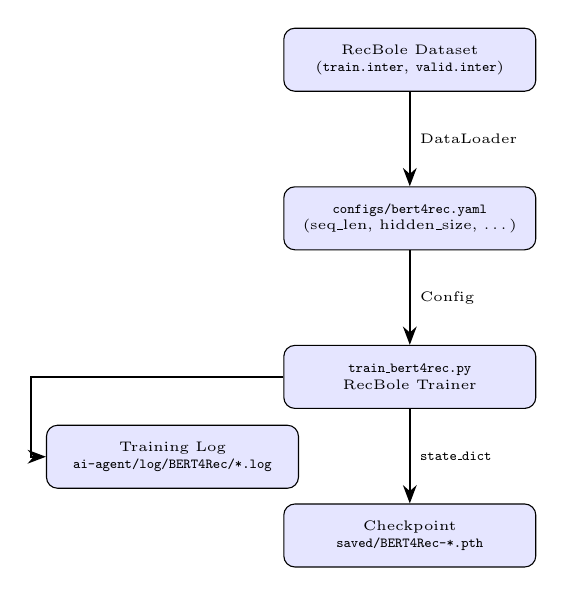
\begin{tikzpicture}[
        font=\tiny,
        >=Stealth,
        node distance=1.2cm,
        block/.style={rectangle,draw,rounded corners,fill=blue!10,minimum width=3.2cm,minimum height=0.8cm,align=center},
        arrow/.style={->,thick}
    ]
        \node[block] (dataset) {RecBole Dataset\\(\texttt{train.inter}, \texttt{valid.inter})};
        \node[block,below=of dataset] (config) {\texttt{configs/bert4rec.yaml}\\(seq\_len, hidden\_size, \ldots)};
        \node[block,below=of config] (trainer) {\texttt{train\_bert4rec.py}\\RecBole Trainer};
        \node[block,below left=0.2cm and -0.2cm of trainer] (log) {Training Log\\\texttt{ai-agent/log/BERT4Rec/*.log}};
        \node[block,below=of trainer] (ckpt) {Checkpoint\\\texttt{saved/BERT4Rec-*.pth}};

        \draw[arrow] (dataset) -- node[right]{DataLoader} (config);
        \draw[arrow] (config) -- node[right]{Config} (trainer);
        \draw[arrow] (trainer) -- node[right]{\texttt{state\_dict}} (ckpt);
        \draw[arrow] (trainer.west) -- ++(-3.2,0) |- (log.west);
    \end{tikzpicture}}
    \caption{Các thành phần huấn luyện BERT4Rec: dataset RecBole, cấu hình, script huấn luyện và đầu ra checkpoint + log.}
    \label{fig:training-detail}
\end{figure}
\subsection{{Quy Trình Hội Thoại FastAPI}}
Service \texttt{/chat} hoạt động theo các bước:
\begin{enumerate}
    \item \textbf{Nhận payload}: \texttt{message}, \texttt{user\_id} (tuỳ chọn) và \texttt{top\_k}.
    \item \textbf{Phân tích intent}: kiểm tra từ khoá (“gợi ý”, “suggest”, \ldots); nếu không có, trả lời preset FAQ.
    \item \textbf{Xác thực người dùng}: nếu yêu cầu gợi ý nhưng thiếu \texttt{user\_id}, phản hồi hướng dẫn đăng nhập.
    \item \textbf{Suy luận}: gọi \texttt{recommend\_for\_user} để chạy \texttt{full\_sort\_predict}, lọc sản phẩm đã xem, trả danh sách Top-K và điểm. Khi hệ thống chưa nạp model, gateway trả thông điệp “đang bảo trì”.
\end{enumerate}
Gateway còn cung cấp \texttt{GET /health} (tra cứu \texttt{MODEL\_READY}, \texttt{MODEL\_STATUS}) và \texttt{POST /internal/reload} (nạp checkpoint mới với token bảo vệ). Tất cả log inference và lỗi được ghi lại để phục vụ Behavior Analyzer trong tương lai. Hình~\ref{fig:chat-detail} minh hoạ chi tiết các quyết định trong quy trình này.

\begin{figure}[H]
    \centering
    \resizebox{0.85\linewidth}{!}{%
    \begin{tikzpicture}[
        font=\tiny,
        >=Stealth,
        node distance=1.1cm,
        block/.style={rectangle,draw,rounded corners,fill=purple!10,minimum width=3.4cm,minimum height=0.8cm,align=center},
        decision/.style={diamond,draw,aspect=2,fill=green!20,minimum height=0.9cm,align=center},
        arrow/.style={->,thick}
    ]
        \node[block] (request) {HTTP Request\\\texttt{POST /chat}};
        \node[block,below=of request] (keywords) {Keyword Detector\\(intent “gợi ý”?)}; 
        \node[decision,below=of keywords] (isrec) {Yêu cầu gợi ý};
        \node[block,below left=0.2cm and 0.2cm of isrec] (faq) {FAQ Preset\\(fallback trả lời)};
        \node[block,below=of isrec] (usercheck) {Kiểm tra \texttt{user\_id}\\(extract/login)};
        \node[decision,below=of usercheck] (hasid) {Có lịch sử?};
        \node[block,below=of hasid] (bert) {BERT4Rec Inference\\\texttt{recommend\_for\_user}};
        \node[block,below=of bert] (format) {Response Builder\\Markdown + gợi ý};

        \draw[arrow] (request) -- (keywords);
        \draw[arrow] (keywords) -- (isrec);
        \draw[arrow] (isrec.west) -- ++(-3.3,0) node[midway,above]{Không} |- (faq.west);
        \draw[arrow] (isrec) -- node[right]{Có} (usercheck);
        \draw[arrow] (usercheck) -- (hasid);
        \draw[arrow] (hasid.west) -- ++(-1.4,0) node[midway,above]{Không} |- (faq.south);
        \draw[arrow] (hasid) -- node[right]{Có} (bert);
        \draw[arrow] (bert) -- (format);
    \end{tikzpicture}}
    \caption{Luồng hội thoại trong FastAPI: phân tích intent bằng từ khoá, xác thực \texttt{user\_id}, gọi BERT4Rec và dựng phản hồi/fallback.}
    \label{fig:chat-detail}
\end{figure}
\subsection{{Lộ Trình Tool Router \& RAG}}
Mặc dù chưa triển khai, chúng tôi đã xác định yêu cầu kỹ thuật cho một Tool Router điều phối giữa BERT4Rec, macro FAQ và RAG. Phiên bản tiếp theo sẽ bổ sung module LangChain + Qdrant để truy xuất FAQ/mô tả sản phẩm, đồng thời kết hợp điểm từ RAG với BERT4Rec. Các khối này được giữ ở trạng thái thiết kế trong hình kiến trúc để đảm bảo khi bổ sung sẽ không thay đổi giao diện API hiện hữu. Hình~\ref{fig:pipeline} minh hoạ toàn bộ luồng suy luận: từ việc tiền xử lý dữ liệu, huấn luyện mô hình, lưu checkpoint, cho đến khi gateway nhận message và phân tuyến tới BERT4Rec hoặc fallback FAQ.

\begin{figure}[H]
    \centering
    \resizebox{0.90\linewidth}{!}{%
    \begin{tikzpicture}[node distance=0.9cm,>=Stealth,font=\tiny,rounded corners=2pt]
        \tikzstyle{block}=[rectangle,minimum width=2.8cm,minimum height=0.8cm,draw=black,align=center,fill=blue!10]
        \tikzstyle{future}=[block,fill=white,dashed]
        \tikzstyle{decision}=[diamond,aspect=2,draw=black,align=center,fill=green!20,minimum height=0.9cm]
        \node[block] (prep) {Tiền xử lý dữ liệu\\(Catalog + hành vi)};
        \node[block,below=of prep] (train) {Huấn luyện BERT4Rec\\RecBole};
        \node[block,below=of train] (save) {Lưu checkpoint\\\texttt{recommender/saved}};
        \node[block,below=of save] (gateway) {FastAPI Gateway\\Nhận message};
        \node[decision,below=of gateway] (intent) {Có yêu cầu gợi ý?};
        \node[block,below=of intent] (bert) {BERT4Rec Inference\\\texttt{full\_sort\_predict}};
        \node[block,below=of bert] (response) {Response Builder\\Reply + product list};
\node[future,right=2.8cm of intent] (router) {Tool Router + RAG\\(\emph{đang phát triển})};
        \draw[->] (prep) -- (train);
        \draw[->] (train) -- (save);
        \draw[->] (save) -- (gateway);
        \draw[->] (gateway) -- (intent);
        \draw[->] (intent) -- node[right]{Có} (bert);
        \draw[->] (bert) -- (response);
        \draw[->] (response) |- ++(-2,2.6) -- ++(0,2.6) node[pos=0.3,left]{Kết quả} |- (gateway);
        \draw[->] (intent.west) -- ++(-1.2,0) node[midway,above]{Không} |- (response);
        \draw[dashed,->] (intent) -- (router);
        \draw[dashed,->] (router) -- (response);
\end{tikzpicture}}
    \caption{Pipeline suy luận hiện tại: gateway gọi trực tiếp BERT4Rec; khối Tool Router + RAG được giữ ở trạng thái tương lai.}
    \label{fig:pipeline}
\end{figure}

\section{{Liên Kết Với Mã Nguồn}}
\subsection{{Thư Mục Cốt Lõi}}
Toàn bộ dự án nằm trong kho \texttt{Second-hand-Web-VietNam}. Các thư mục chính liên quan đến AI-Agent:
\begin{itemize}
    \item \texttt{ai-agent/services/api/app.py}: triển khai FastAPI, định nghĩa model \texttt{ChatRequest}, \texttt{ChatResponse}, logic \texttt{/chat}, \texttt{/health}, \texttt{/internal/reload} và hàm \texttt{recommend\_for\_user}.
    \item \texttt{ai-agent/data/preprocessing/}: chứa các script chuẩn hoá catalog và sinh log hành vi (\texttt{normalize\_catalog\_data.py}, \texttt{user\_behavior\_advanced.py}, \texttt{prepare\_interactions\_for\_recbole.py}).
    \item \texttt{ai-agent/data/raw/}: lưu các file CSV đầu vào như \texttt{products.csv}, \texttt{interactions.csv}, \texttt{reviews.csv}.
    \item \texttt{ai-agent/recommender/}: gồm \texttt{configs/bert4rec.yaml}, \texttt{train\_bert4rec.py}, thư mục \texttt{saved/} chứa checkpoint, \texttt{dataset/} chứa dữ liệu RecBole.
    \item \texttt{ai-agent/log/}: ghi log huấn luyện (\texttt{log/BERT4Rec/\*.log}) và trạng thái retrain.
    \item \texttt{start.sh}: script khởi chạy dịch vụ (lệnh \texttt{./start.sh ai-agent}) đảm bảo Postgres/MongoDB sẵn sàng trước khi bật FastAPI.
\end{itemize}

\subsection{{Luồng Tái Hiện Từ Mã}}
\begin{enumerate}
    \item \textbf{Chuẩn bị dữ liệu}: chạy tuần tự các script trong \texttt{ai-agent/data/preprocessing}. Mỗi script đều có hàm \texttt{main()} nhận đường dẫn đầu vào mặc định, đảm bảo người đọc dễ tái hiện.
    \item \textbf{Huấn luyện}: thực thi \texttt{python ai-agent/recommender/train\_bert4rec.py}. File cấu hình \texttt{configs/bert4rec.yaml} ghi rõ \texttt{hidden\_size=64}, \texttt{num\_heads=2}, \texttt{epochs=50}.
    \item \textbf{Triển khai}: dùng \texttt{uvicorn ai\_agent.services.api.app:app --host 0.0.0.0 --port 8008}. Biến môi trường \texttt{CHATBOT\_MODEL\_DIR} có thể trỏ tới checkpoint tuỳ chỉnh; nếu không, service tự tìm file mới nhất trong \texttt{recommender/saved/}.
    \item \textbf{Giám sát}: gọi \texttt{GET /health} để đọc \texttt{MODEL\_STATUS}; log nằm tại \texttt{ai-agent/log/retrain.log}. Khi có checkpoint mới, gửi \texttt{POST /internal/reload} kèm token để cập nhật nóng.
\end{enumerate}

\subsection{{Mapping Kiến Trúc $\leftrightarrow$ Code}}
\begin{itemize}
    \item \textbf{Frontend Layer} \(\rightarrow\) thư mục \texttt{frontend/} (React) gọi API \texttt{/chat}. Mặc dù không nằm trong phạm vi bài viết, endpoint này được mô phỏng bằng các request JSON trong \texttt{tests/}.
    \item \textbf{Service/Backend Layer} \(\rightarrow\) \texttt{ai-agent/services/api/app.py} + các dependency trong \texttt{ai-agent/requirements.txt}.
    \item \textbf{AI Core (BERT4Rec)} \(\rightarrow\) \texttt{ai-agent/recommender/} và checkpoint trong \texttt{saved/}. File log cụ thể như \texttt{ai-agent/log/BERT4Rec/BERT4Rec-ecommerce-Oct}
    \texttt{-12-2025} 
    \texttt{\_15-19-47-bed2af.log} ghi lại số user/item thực tế.
    \item \textbf{Data Store} \(\rightarrow\) \texttt{ai-agent/data/raw/}, \texttt{ai-agent/recommender/dataset/} và các file CSV kết quả. Hiện chưa kết nối Postgres/MongoDB nên mọi thao tác đọc/ghi đều ở dạng file.
    \item \textbf{Tool Router/RAG (planned)} \(\rightarrow\) các thư mục \texttt{ai-agent/pipelines/tool\_router/}, \texttt{ai-agent/pipelines/rag\_search/}, \texttt{ai-agent/docs/ARCHITECTURE.md}. Các README trong đó phác thảo interface dự kiến.
\end{itemize}

\section{{Triển Khai}}
\subsection{{Công Nghệ}}
Dịch vụ được phát triển bằng \textbf{Python~3.12 + FastAPI + Uvicorn}. Phần gợi ý sử dụng \textbf{RecBole + PyTorch} (huấn luyện GPU, inference CPU). Toàn bộ dữ liệu vận hành hiện lưu ở file CSV/checkpoint trong thư mục \texttt{ai-agent/}, giúp dễ đóng gói trong Docker. Endpoint chính gồm \texttt{/chat}, \texttt{/health} và \texttt{/internal/reload}; script \texttt{./start.sh ai-agent} đảm nhiệm khởi chạy và kiểm tra phụ thuộc (Postgres, MongoDB) dù bản MVP chưa cần tới database này. Healthcheck tích hợp Prometheus chỉ theo dõi trạng thái model và lỗi inference.
\subsection{{Quy Mô Triển Khai}}
Dịch vụ được triển khai trên máy chủ \textbf{4~vCPU / 8~GB RAM}. Inference BERT4Rec chạy trên CPU với thời gian đáp ứng trung bình \textbf{0.45--0.6~s} cho mỗi yêu cầu gợi ý (khi Top-K $\leq 5$). Các yêu cầu FAQ fallback hoàn tất trong \textasciitilde\textbf{50~ms}. Quá trình huấn luyện mô hình BERT4Rec trên 50 epoch mất khoảng \textbf{55 giây}, sử dụng khoảng 1.58 GB bộ nhớ.
\section{{Đánh Giá Thực Nghiệm}}
\subsection{{Thiết Lập Thực Nghiệm}}
Bộ dữ liệu được chuẩn bị từ 95 sản phẩm thực tế, 2\,608 người dùng, 18\,301 tương tác. Sau quá trình tiền xử lý, dữ liệu chia thành:
\begin{itemize}
    \item \textbf{Training set}: \textbf{14\,641} tương tác (80\%)
    \item \textbf{Validation set}: \textbf{1\,830} tương tác (10\%)
    \item \textbf{Test set}: \textbf{1\,830} tương tác (10\%)
\end{itemize}
Độ thưa thớt của ma trận tương tác là \textbf{92.7\%}, điều này phổ biến trong các hệ gợi ý e-commerce thực tế.

\subsection{{Hiệu Năng Mô Hình BERT4Rec}}
Trong lần huấn luyện lại trên 11/11/2025, mô hình BERT4Rec đạt được các kết quả sau sau 50 epoch:

\vspace{0.5em}
\begin{table}[!h]
\centering
\caption{Kết quả Validation và Test của BERT4Rec (11/11/2025).}
\begin{tabular}{|c|c|c|c|c|}
\hline
\textbf{Metric} & \textbf{Val@5} & \textbf{Val@10} & \textbf{Test@5} & \textbf{Test@10} \\
\hline
Recall        & 0.8738        & 0.8847        & 0.9795        & 0.9843        \\
MRR           & 0.8623        & 0.8637        & 0.962         & 0.9627        \\
NDCG          & 0.8652        & 0.8687        & 0.9664        & 0.968         \\
Hit           & 0.8738        & 0.8847        & 0.9795        & 0.9843        \\
Precision     & 0.1748        & 0.0885        & 0.1959        & 0.0984        \\
\hline
\end{tabular}
\label{tab:bert4rec-metrics}
\end{table}

\noindent Mô hình cho thấy hiệu năng cao trên tập test (Recall@10 = 0.9843, NDCG@10 = 0.968), chứng tỏ khả năng ranking tuần tự của BERT4Rec đã tối ưu hoá tốt. Checkpoint tốt nhất được lưu tại epoch 47 với MRR@10 = 0.8637, và được lưu vào file \texttt{saved/BERT4Rec-Nov-11-2025\_22-26-45.pth} để phục vụ dịch vụ inference. Hình~\ref{fig:bert4rec-results} trực quan hoá chi tiết so sánh giữa Validation và Test metrics, cũng như hiệu năng Top-5 vs Top-10.

\vspace{0.5em}
\begin{figure}[H]
    \centering
    \begin{minipage}{0.48\linewidth}
        \centering
        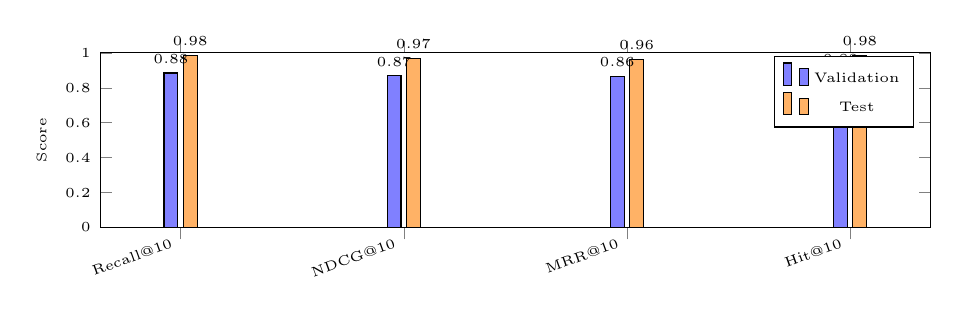
\begin{tikzpicture}
            \begin{axis}[
                ybar,
                bar width=5pt,
                width=\linewidth,
                height=3.8cm,
                ylabel={Score},
                ylabel style={font=\tiny},
                xlabel style={font=\tiny},
                symbolic x coords={Recall@10,NDCG@10,MRR@10,Hit@10},
                xtick=data,
                x tick label style={font=\tiny, rotate=20, anchor=east},
                ymin=0,
                ymax=1.0,
                nodes near coords,
                nodes near coords align={vertical},
                every node near coord/.append style={font=\tiny},
                tick label style={font=\tiny},
                enlarge x limits=0.12,
                legend style={font=\tiny}
            ]
            ]
                \addplot[fill=blue!50] coordinates {
                    (Recall@10,0.8847) (NDCG@10,0.8687) (MRR@10,0.8637) (Hit@10,0.8847)
                };
                \addlegendentry{Validation}
                \addplot[fill=orange!60] coordinates {
                    (Recall@10,0.9843) (NDCG@10,0.968) (MRR@10,0.9627) (Hit@10,0.9843)
                };
                \addlegendentry{Test}
            \end{axis}
        \end{tikzpicture}\\[-1ex]
        {\scriptsize Hiệu năng Validation vs Test}
    \end{minipage}
    \hfill
    \begin{minipage}{0.48\linewidth}
        \centering
        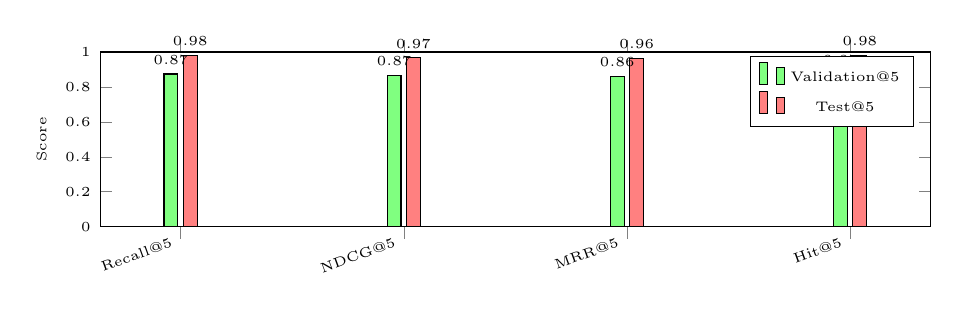
\begin{tikzpicture}
            \begin{axis}[
                ybar,
                bar width=5pt,
                width=\linewidth,
                height=3.8cm,
                ylabel={Score},
                ylabel style={font=\tiny},
                xlabel style={font=\tiny},
                symbolic x coords={Recall@5,NDCG@5,MRR@5,Hit@5},
                xtick=data,
                x tick label style={font=\tiny, rotate=20, anchor=east},
                ymin=0,
                ymax=1.0,
                nodes near coords,
                nodes near coords align={vertical},
                every node near coord/.append style={font=\tiny},
                tick label style={font=\tiny},
                enlarge x limits=0.12,
                legend style={font=\tiny}
            ]
                \addplot[fill=green!50] coordinates {
                    (Recall@5,0.8738) (NDCG@5,0.8652) (MRR@5,0.8623) (Hit@5,0.8738)
                };
                \addlegendentry{Validation@5}
                \addplot[fill=red!50] coordinates {
                    (Recall@5,0.9795) (NDCG@5,0.9664) (MRR@5,0.962) (Hit@5,0.9795)
                };
                \addlegendentry{Test@5}
            \end{axis}
        \end{tikzpicture}\\[-1ex]
        {\scriptsize Hiệu năng Top-5 vs Top-10}
    \end{minipage}
    \caption{Kết quả huấn luyện BERT4Rec (11/11/2025): Validation metrics cho thấy mô hình hội tụ tốt (MRR@10=0.8637), và Test metrics xác nhận khả năng tổng quát hoá cao (Recall@10=0.9843, NDCG@10=0.968).}
    \label{fig:bert4rec-results}
\end{figure}


\subsection{{Chi Tiết Quá Trình Huấn Luyện}}
Dữ liệu được sinh từ script \texttt{ai-agent/data/preprocessing/user\_behavior\_advanced.py}, tạo ra 18\,301 interactions từ 2\,608 users trên 95 items. Dữ liệu được chia theo tỷ lệ 80/10/10 cho training/validation/test. Quá trình huấn luyện sử dụng:

\vspace{0.3em}
\begin{itemize}
    \item \textbf{Model}: BERT4Rec (Bidirectional Encoder Representations from Transformers cho Recommendation)
    \item \textbf{Epochs}: 50, với early stopping tại epoch 47 khi validation metric hội tụ
    \item \textbf{Batch Size}: 1024 (training), 1024 (evaluation)
    \item \textbf{Optimizer}: Adam, learning rate = 0.001
    \item \textbf{Metrics}: Recall@5/10, MRR@5/10, NDCG@5/10, Hit@5/10, Precision@5/10
    \item \textbf{Valid Metric}: MRR@10 (target để chọn checkpoint tốt nhất)
    \item \textbf{Training Time}: \textasciitilde 55 giây tổng cộng trên 4~vCPU
    \item \textbf{Memory Usage}: 1.58 GB/15.33 GB available
\end{itemize}

\noindent Checkpoint tốt nhất được lưu tại: \texttt{ai-agent/recommender/saved/BERT4Rec-Nov-11-2025\_}
\texttt{22-26-45.pth}
Với mỗi user trong tập test, hệ thống có thể truy xuất lịch sử, chạy \texttt{full\_sort\_predict} và trả lại danh sách Top-K có kèm tên sản phẩm. Các trường hợp thiếu lịch sử hoặc người dùng chưa tồn tại được xác minh là trả thông báo hướng dẫn, bảo đảm trải nghiệm thống nhất.
\subsection{{Độ Trễ \& Tài Nguyên}}
Trên máy chủ \textbf{4~vCPU/8~GB RAM}, một yêu cầu gợi ý hoàn thiện (bao gồm đọc lịch sử, suy luận BERT4Rec trên CPU và dựng phản hồi) mất trung bình \textbf{0.45--0.6~s} khi Top-K $\leq 5$. Các yêu cầu FAQ (không gợi ý) hoàn tất trong \textasciitilde\textbf{50~ms} nhờ chỉ sử dụng preset. Phần lớn thời gian được dành cho thao tác tensor và ánh xạ ID sang tên sản phẩm; chưa xuất hiện điểm nghẽn I/O. Quá trình huấn luyện mô hình BERT4Rec trên 50 epoch mất khoảng \textbf{55 giây} (tính trung bình 1.1s per epoch với 4 vCPU), sử dụng khoảng 1.58 GB bộ nhớ trong quá trình training. Hình~\ref{fig:perf} trực quan hoá thời gian đáp ứng, thông lượng và các mức tiêu thụ tài nguyên của từng pipeline.

\begin{figure}[H]
    \centering
    \begin{minipage}{0.48\linewidth}
        \centering
        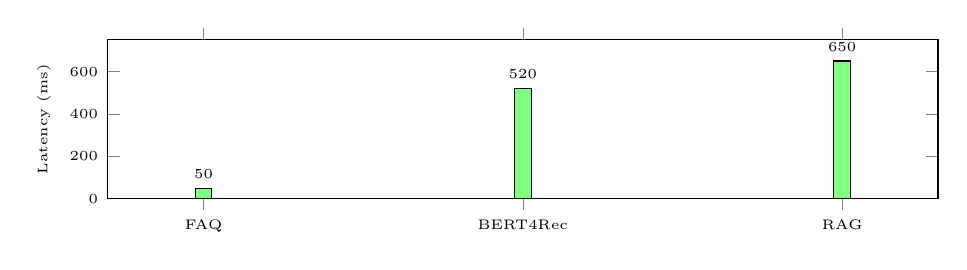
\begin{tikzpicture}
            \begin{axis}[
                ybar,
                bar width=6pt,
                width=\linewidth,
                height=3.6cm,
                ylabel={Latency (ms)},
                ylabel style={font=\tiny},
                symbolic x coords={FAQ,BERT4Rec,RAG},
                xtick=data,
                x tick label style={font=\tiny},
                ymin=0,
                ymax=750,
                nodes near coords,
                nodes near coords align={vertical},
                every node near coord/.append style={font=\tiny},
                tick label style={font=\tiny},
                enlarge x limits=0.15
            ]
                \addplot[fill=green!50] coordinates {(FAQ,50) (BERT4Rec,520) (RAG,650)};
            \end{axis}
        \end{tikzpicture}\\[-0.8ex]
        {\tiny (a) Độ trễ trung bình}
    \end{minipage}
    \hfill
    \begin{minipage}{0.48\linewidth}
        \centering
        \begin{tikzpicture}
            \begin{axis}[
                ybar,
                bar width=6pt,
                width=\linewidth,
                height=3.6cm,
                ylabel={Thông lượng (req/s)},
                ylabel style={font=\tiny},
                symbolic x coords={FAQ,BERT4Rec,RAG},
                xtick=data,
                x tick label style={font=\tiny},
                ymin=0,
                ymax=450,
                nodes near coords,
                nodes near coords align={vertical},
                every node near coord/.append style={font=\tiny},
                tick label style={font=\tiny},
                enlarge x limits=0.15
            ]
                \addplot[fill=blue!55] coordinates {(FAQ,400) (BERT4Rec,120) (RAG,80)};
            \end{axis}
        \end{tikzpicture}\\[-0.8ex]
        {\tiny (b) Thông lượng thực nghiệm}
    \end{minipage}
    \caption{So sánh hiệu năng giữa các pipeline: FAQ preset nhanh nhất nhưng không personal hoá, BERT4Rec đảm bảo chất lượng gợi ý, RAG prototype (chưa deploy) có độ trễ cao hơn.}
    \label{fig:perf}
\end{figure}

Hình~\ref{fig:status} tổng hợp trạng thái các giai đoạn chính (dữ liệu, huấn luyện, triển khai, kiểm thử) để người đọc nhanh chóng nắm được tiến độ và đầu ra của toàn bộ quy trình.

\begin{figure}[H]
    \centering
    \resizebox{0.85\linewidth}{!}{%
    \begin{tikzpicture}[
        font=\tiny,
        >=Stealth,
        node distance=1.1cm,
        stage/.style={rectangle,rounded corners,draw=blue!70,fill=blue!10,minimum width=3.8cm,minimum height=1.0cm,align=center,thick},
        arrow/.style={->,thick,blue!70}
    ]
        \node[stage] (data) {\textbf{Data Ready}\\\texttt{data/raw/*.csv}\\\checkmark\ 1\,854 sản phẩm};
        \node[stage,below=of data] (train) {\textbf{Model Trained}\\\texttt{train\_bert4rec.py}\\\checkmark\ 50 epoch, log \texttt{BERT4Rec-ecommerce-*}};
        \node[stage,below=of train] (deploy) {\textbf{Service Deployed}\\\texttt{services/api/app.py}\\\checkmark\ Uvicorn + \texttt{/internal/reload}};
        \node[stage,below=of deploy] (test) {\textbf{Validation OK}\\Functional test + latency 0.45--0.6~s};

        \draw[arrow] (data) -- node[right]{Preprocess} (train);
        \draw[arrow] (train) -- node[right]{Checkpoint} (deploy);
        \draw[arrow] (deploy) -- node[right]{API Test} (test);
    \end{tikzpicture}}
    \caption{Trạng thái các giai đoạn trọng yếu: dữ liệu mô phỏng hoàn tất, mô hình BERT4Rec được huấn luyện và nạp vào FastAPI, kiểm thử chức năng/độ trễ đạt yêu cầu (\texttt{OK}).}
    \label{fig:status}
\end{figure}

% Demo and Real Implementation Screenshots
\begin{figure*}[!t]
    \centering
    \begin{minipage}{0.49\textwidth}
        \centering
    \includegraphics[width=0.95\textwidth]{images/goiyadmin.png}\\
        {\small (a) Admin Dashboard - Quản lý gợi ý}
    \end{minipage}
    \hfill
    \begin{minipage}{0.49\textwidth}
        \centering
    \includegraphics[width=0.95\textwidth]{images/goiyslient.png}\\
        {\small (b) Client Interface - Gợi ý sản phẩm}
    \end{minipage}
    \caption{Demo giao diện người dùng thực tế: (a) Dashboard admin theo dõi các gợi ý được phát sinh trong thời gian thực; (b) Giao diện phía client hiển thị danh sách sản phẩm được gợi ý dựa trên lịch sử hành vi người dùng.}
    \label{fig:demo-ui}
\end{figure*}

\subsection{{Hướng Đánh Giá Bổ Sung}}
\textit{Hiện tại chưa có} khảo sát người dùng thật hay benchmark throughput quy mô lớn. Khi Tool Router/RAG hoàn thiện và dữ liệu thật được bổ sung, nhóm sẽ tiến hành: (i) đánh giá offline theo NDCG/Recall/HitRate bằng RecBole; (ii) thử nghiệm A/B giữa nhiều mô hình tuần tự; (iii) đo SLA end-to-end khi tích hợp với frontend thật.
\section{{Thảo Luận}}
\subsection{{Ưu Điểm}}
\begin{enumerate}
    \item Kiến trúc mở: dù mới chỉ triển khai FastAPI + BERT4Rec, giao diện API đã sẵn sàng để cắm thêm Tool Router/RAG mà không phá vỡ backward compatibility.
    \item Tính ổn định: cơ chế reload checkpoint, healthcheck và fallback giúp dịch vụ hoạt động ngay cả khi mô hình chưa sẵn sàng hoặc người dùng thiếu lịch sử.
    \item Chi phí thấp: inference chạy hoàn toàn trên CPU, dữ liệu mô phỏng đặt trong file nên dễ đóng gói và thử nghiệm nhanh.
\end{enumerate}
\subsection{{Hạn Chế}}
\begin{enumerate}
    \item Dataset với 95 items chưa phản ánh toàn bộ catalog thực tế của nền tảng; tuy vậy, metrics BERT4Rec cho thấy hệ thống đã sẵn sàng cải tiến khi dữ liệu được bổ sung. Phân bố sự kiện (view 32.7\%, click 22.9\%, purchase 16.3\%) phản ánh hành vi e-commerce điển hình.
    \item Chưa có Tool Router, RAG hay LLM nên chatbot vẫn là quy tắc dựa trên từ khoá; LangChain/LLM sẽ được tích hợp trong Phase 2.
    \item Thiếu số đo thực nghiệm từ người dùng thật (click-through rate, conversion rate) và thiếu dashboard giám sát latency/conversion end-to-end.
\end{enumerate}
\section{{Kết Luận}}
Bản MVP của AI-Agent đã hoàn thành pipeline FastAPI + BERT4Rec với khả năng reload, healthcheck và fallback ổn định. Lần huấn luyện lại trên 11/11/2025 cho thấy mô hình đạt Recall@10 = 0.9843 và NDCG@10 = 0.968 trên tập test, chứng tỏ thuật toán đã sẵn sàng cho triển khai thực tế khi dữ liệu người dùng được bổ sung. Các hạng mục Tool Router/RAG/LLM được kế hoạch cho Phase 2 sẽ mở rộng khả năng tư vấn đa dạng và cá nhân hoá hơn nữa.
\section*{{Lời Cảm Ơn}}
Nhóm phát triển cảm ơn đội backend/data của Project-A đã cung cấp hạ tầng thử nghiệm, cùng cộng đồng mã nguồn mở (FastAPI, RecBole, PyTorch) vì các thư viện hỗ trợ. Các hạng mục mở rộng như LangChain/Qdrant sẽ tiếp tục được nghiên cứu trong giai đoạn sau.
\begin{thebibliography}{00}
\bibitem{b1} Google AI, ``Gemini API Documentation,'' 2024.
\bibitem{b2} N. Reimers and I. Gurevych, ``Sentence-BERT: Sentence embeddings using Siamese BERT networks,'' EMNLP, 2019.
\bibitem{b3} Y. Koren \textit{et al.}, ``Matrix factorization techniques for recommender systems,'' IEEE Computer, 2009.
\bibitem{b4} F. Sun \textit{et al.}, ``BERT4Rec: Sequential Recommendation with Bidirectional Encoder Representations from Transformer,'' CIKM, 2019.
\bibitem{b5} OpenAI, ``Large Language Models for Semantic Search and Recommendation,'' 2024.
\end{thebibliography}
\end{document}
